
\documentclass{article}
\usepackage[utf8]{inputenc}

\usepackage{amsthm}
\usepackage{amsmath}
\newtheoremstyle{mystyle}% name
  {\topsep}% Space above
  {\topsep}% Space below
  {\normalfont}% Body font
  {}% Indent amount
  {\bfseries}% Theorem head font
  {}%Punctuation after theorem head
  {.5em}%Space after theorem head
  {}% theorem head spec
\theoremstyle{mystyle}
\newtheorem{prob}{Problem}
\usepackage{graphicx}
\usepackage{wrapfig}


\title{EN.520.216 Homework 1}
\author{LJ Gonzales}
\date{February 2023}

\begin{document}
\maketitle
\section{Manufacturing Problems}
\begin{prob}
\begin{enumerate} 
	\item On the wafer "length" of 36L, we can have at most $\lfloor\frac{3\times10^{-3}}{36\times90\times10^{-9}/2}\rfloor=1851$ "rows" of transistors and $\lfloor\frac{3\times10^{-3}}{24\times90\times10^{-9}/2}\rfloor=2777$ "columns", for a total of 5,140,227 transistors. This makes the assumption that transistors are allowed to be side-to-side with no space between them (or that the necessary space is included in the provided area). Also, we assume the chip is single-layer.
\item Same as the previous, 5,140,227 transistors. Another assumption we need to make is that both n-mos and p-mos transistors are the same size, which I believe would not be normal practice. Also, there will be more parasitic effects like leakage current compared to FD-SOI because the insulator layer on an SOI wafer isolates different transistors from affecting each other, unlike CMOS which is bulked together.
\item With a similar computation as the previous problems, we find that $\lfloor\frac{3\times10^{-3}}{36\times130\times10^{-9}/2}\rfloor=1282$ "rows" of transistors and $\lfloor\frac{3\times10^{-3}}{24\times130\times10^{-9}/2}\rfloor=1923$ "columns", for a total of 2,465,286 transistors.  
\end{enumerate}
\end{prob}

\section{Device Physics Problems}
\begin{prob}
\begin{enumerate}
    \item The Fermi function gives the probability that a state \emph{at a given energy} is filled with an electron. Because the total amount of available states at a given energy is large, this is basically equivalent to the fraction of states that are filled by an electron.
\item We use the Fermi function \[f(E)=\frac{1}{1+e^{(E-E_f)/kT}}\] with $E=E_f+0.225kT$, giving $\frac{1}{1+e^{0.225/(8.6\times10^{-5}\times325}}\approx3.1\times10^{-4}$.
    \item Again use the Fermi function \[f(E)=\frac{1}{1+e^{(E-E_f)/kT}}\] with $E=E_f+10kT$, giving $\frac{1}{1+e^{10/(8.6\times10^{-5}\times325}}\approx4.14\times10^{-156}$, which is essentially 0.
    \item The fermi level does not shift as a function of temperature. However, increasing the temperature does decrease the 'sensitivity' to small changes in energy around the fermi level. At 0K, we assume a small decrease in energy bring the fermi level to 1 and a small increase to bring it down all the way to 0, but at higher temperatures the transition is more subtle. Decreasing the temperature would then be desirable in digital circuits because you can make much easier to calculate assumptions about the circuit's states.
\end{enumerate}
\end{prob}

\begin{prob}
	\begin{enumerate}
		\item We know that $n_i\approx\int_{E_c}^{\infty}g(E)e^{\frac{E-E_{fi}}{kT}}dE$ and $n_d\approx\int_{E_c}^{\infty}g(E)e^{\frac{E-E_{fd}}{kT}}dE$. Note we make the assumption that the  energy levels we're integrating over is larger than the fermi level+3kT, which is to be expected. But now if we just call $E_{fd}=E_{fi}+\Delta E$ where E is just some constant that represents how far the doped fermi level is relative to the intrinsic fermi level, we find that:  
	\[\begin{split} 
		\frac{n_i}{n_d}=\frac{\int_{E_c}^{\infty}g(E)e^{\frac{E-E_{fi}}{kT}}dE}{\int_{E_c}^{\infty}g(E)e^{\frac{E-(E_{fi}+\Delta E)}{kT}}dE} \\
    =\frac{1}{e^{- \Delta E/kT}}\frac{\int_{E_c}^{\infty}g(E)e^{\frac{E-E_{fi}}{kT}}dE}{\int_{E_c}^{\infty}g(E)e^{\frac{E-E_{fi}}{kT}}dE}=\frac{1}{e^{-\Delta E/kT}} \\
 \therefore \ln{\frac{10^{10}}{10^{17}}} = \frac{-\Delta E}{kt} \\
	\end{split} 
 \]

From this we substitute our known values of k and T, $8.6\times10^{-5}$ and $295$, respectively, to find that $\Delta E\approx0.409$, in other words the Fermi level is 0.409eV above the intrinsic fermi level of 1.1eV, for a total of about 1.5eV. 

        \item 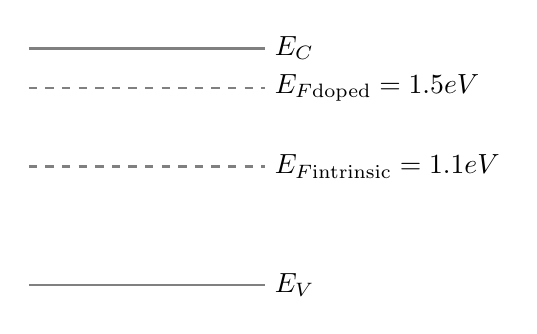
\begin{tikzpicture}
        \draw[gray, thick] (-1,3) -- (2,3);
        \node[right] at (2,3) {$E_C$};
        \draw[gray, thick, dashed] (-1,2.5) -- (2,2.5);
        \node[right] at (2,2.5) {$E_{F\text{doped}}=1.5eV$};
        \draw[gray, thick, dashed] (-1,1.5) -- (2,1.5);
        \node[right] at (2,1.5) {$E_{F\text{intrinsic}}=1.1eV$};
        \draw[gray, thick] (-1,0) -- (2,0);
        \node[right] at (2,0) {$E_V$};
        \end{tikzpicture}

        \item The acceptor concentration can be calculated from the additional assumption $p=N_A$ and the law of mass action $np=n_i^2$, such that $N_A=p=\frac{(10^{10})^2}{10^{17}}=10^3$ acceptors/cm3
    \end{enumerate}
\end{prob}

\begin{prob}
\begin{enumerate}
	\item With the same formula as before $\Delta E=-kt\ln\frac{n_i}{n}$, and the assumption $n=N_D$, we find the separation to be 0.178eV (up relative to the intrinsic fermi level). 
	\item Here we need to first find the concentration of electrons as a result of this doping before inserting in the same equation. We find that $n=\frac{n_i^2}{N_A}=\frac{(10^{10})^2}{5\times10^{14}}=0.2\times10^6$ hence :$\Delta E=-kt\ln\frac{10^{10}}{0.2\times10^6}=-0.279$eV. As expected the fermi level decreases.
	\item We take the value of n used in computation to get $n=0.2\times10^6$ electrons/$cm^3$
\end{enumerate}
\end{prob}

\end{document}
